% Straight up stealing preamble from Eli Holmes 
%%%%%%%%%%%%%%%%%%%%%%%%%%%%%%%%%%%%%%START PREAMBLE THAT IS THE SAME FOR ALL EXAMPLES
\documentclass{article}

%Required: You must have these
\usepackage{Sweave}
\usepackage{graphicx}
\usepackage{tabularx}
\usepackage{hyperref}
\usepackage{natbib}
\usepackage{pdflscape}
\usepackage{array}
\usepackage{gensymb}
%\usepackage[backend=bibtex]{biblatex}
%Strongly recommended
  %put your figures in one place
%\SweaveOpts{prefix.string=figures/, eps=FALSE} 
%you'll want these for pretty captioning
\usepackage[small]{caption}

\setkeys{Gin}{width=0.8\textwidth}  %make the figs 50 perc textwidth
\setlength{\captionmargin}{30pt}
\setlength{\abovecaptionskip}{10pt}
\setlength{\belowcaptionskip}{10pt}
% manual for caption  http://www.dd.chalmers.se/latex/Docs/PDF/caption.pdf

%Optional: I like to muck with my margins and spacing in ways that LaTeX frowns on
%Here's how to do that
 \topmargin -1.5cm        
 \oddsidemargin -0.04cm   
 \evensidemargin -0.04cm  % same as oddsidemargin but for left-hand pages
 \textwidth 16.59cm
 \textheight 21.94cm 
 %\pagestyle{empty}       % Uncomment if don't want page numbers
 \parskip 7.2pt           % sets spacing between paragraphs
 %\renewcommand{\baselinestretch}{1.5} 	% Uncomment for 1.5 spacing between lines
\parindent 0pt% sets leading space for paragraphs
\usepackage{setspace}
%\doublespacing

%Optional: I like fancy headers
%\usepackage{fancyhdr}
%\pagestyle{fancy}
%\fancyhead[LO]{How do climate change experiments actually change climate}
%\fancyhead[RO]{2016}
 
%%%%%%%%%%%%%%%%%%%%%%%%%%%%%%%%%%%%%%END PREAMBLE THAT IS THE SAME FOR ALL EXAMPLES

%Start of the document
\begin{document}

%\SweaveOpts{concordance=TRUE}
 \bibliographystyle{/Users/aileneettinger/citations/Bibtex/styles/amnat.bst}
\title{Spatial and temporal shifts in photoperiod with climate change} % perspective paper for OSPREE analyses

\author{A.K. Ettinger, D. Buonaiuto, C. Chamberlain, I. Morales-Castilla, E. Wolkovich}
%\date{\today}%do we need to also add any of the following: D. Flynn, T. Savas, J. Samaha, E. Forrestel? 
\maketitle  %put the fancy title on
%\tableofcontents      %add a table of contents
%\clearpage
%%%%%%%%%%%%%%%%%%%%%%%%%%%%%%%%%%%%%%%%%%%%%%%%%%%

%%%%%%%%%%%%%%%%%%%%%%%%%%%%%%%%%%%%%%%%%%%%%%%%%%%
\iffalse
Lizzie's comments on 22 September 2018

I think this is a great start to the paper and could move quickly to a draft we're polishing. But, as I often find with my papers I am super excited about initially, I think it has lost some of its excitement! I have a couple ideas on how to get it back below ... but a big part will just be trying to revert back to our thinking a year ago... we can all help with that through editing. 

(1) While I like the idea of focusing bigger than plants, I think it could be a hard sell for several reasons:
	(1a) Most of the paper is about the OSPREE database, so that's where we have data and can say the most interesting things.
	(1b) I think the paper lags when we try to discuss insects or salmon or whatnot, it reads more like a textbook in these sections to me, versus an exciting new paper.
	(1c) This doesn't mean we can start and end bigger but I think the paper would be much better off starting big, admitting we focus on plants, then ending with a nod again to other taxa. It could even angle as -- hey, this is plants where we don't even worry as much about photoperiod as we do with other taxa so this is really important!
(
2) I think one thing that may help with our thinking and shaping of the paper is a conceptual figure to end on that tells readers in a flow-diagram way how they should incorporate photoperiod into predictions.... we could do this for several forecasting methods: process-based models, statistical models and species distribution models. We may not need a final or pretty version of the figure for the paper but us all working on it could help shape and strengthen the message of the paper .... More on this below.

(3) We also should add a clear statement of our take-home messages and why they matter and are interesting to help guide us back to that excitement. Here are some that I see:
(*) Temporal shifts are expected to have a major impact on experienced photoperiod, thus testing for the importance of photoperiod to phenology and adding it to such models should be a major goal.
(*) Current experiments often go well beyond the expected spatial and temporal shifts of climate change, especially for the bigger treatments (Fig. 3) but  the smaller treatments seem to overlap with potential shifts (?!) and appear relevant (Fig. 4-5). 
Could/should we add: 
(*) A vote-count to table 1 of which studies found an effect of photoperiod? This could be used early in the paper to suggest whether photoperiod matters and point out the value of such experiments. It would be easy for the lab to help with this task. 
(*) How to predict how much photoperiod matters? Evidence suggests it varies (importantly?) by ... species, lifestage, photoperiod (Fig. 6), population (that is genotype, and this may relate to latitude). 

(4) One thing Cat did for her recent frost paper that helped a lot was outlined 'outstanding questions.' I think we could do that also and we could help write a paper that leads to the ones we identify!

More on models ....
In my mind there are two extremes: statistical models and process-based models. Most statistical models have a little process (that's your predictor variables) and most process-based models have a good dose of statistical (you fit the parameters!). I am thinking most SDMs are statistical so you could toss them as an example under the statistical.

To date in statistical models many people either ignore photoperiod or they put it in in some very painful way ('we added photoperiod experienced on the day of budburst to the PEP725 data to test for the role of photoperiod') that is not well designed. What we're fundamentally suggesting is they step a little in the direction of process-based models and:
(1) Use experimental data (there's lots we have shown in this paper) to test if their species or a congeneric species shows a photoperiod effect (ideally test how it varies by lifestage and genotype)
(2) If there is a response, add this to the model (we could cite some of Isabelle's papers to describe how much it could matter).
(3) What will be critical are non-linearities and/or variations across species, lifestages, and populations -- these could fundamentally shape future species and communities! We could help the reader visualize an example of this.
(4) Models ideally will then guide experiments to test some of the critical predictions ....
	
Some smaller comments below by me are prefaced by %EMW	
\fi
%%%%%%%%%%%%%%%%%%%%%%%%%%%%%%%%%%%%%%%%%%%%%%%%%%%


%%%%%%%%%%%%%%%%%%%%%%%%%%%%%%%%%%%%%%%%
\iffalse
Nacho's comments 10 October 2018

Not sooo much to add to Lizzie's super helpful comments at this stage. Thanks Ailene for putting this together, 
reading it still makes me very excited about the topic, but perhaps we can still make it more appealing. Just a couple comments:
	

- I agree that we should restrict to plants in the intro and leaving the overview of how this paper may be 
important for other taxa to the end. 

- We say that photoperiod matters but not why it matters. Perhaps we should mention that, one reason why photoperiod would matter to plants is that it is directly related with the amount
of photosynthesis a plant can do, thus influencing physiological processes such as growth. This is obviously
important to plants and yet, commonly overlooked in forecasts. We can try to mention this in a non-text book fashion. 

- By the end of paragraph 2 we could add a couple of examples of biological responses (growth, phenology, etc.).

- I like the idea of a section on "outstanding questions". An obvious one coming to mind is: how much does 
model accuracy (process-based or correlational-statistical-SDMs) improve when we account for photoperiod? If 
models do not improve much or not at all, then I guess we could forget about it. However, it is likely that
photoperiod be important for certain taxa, in certain regions and when using certain models, and answering that
is really important, isn't it?

\fi
%%%%%%%%%%%%%%%%%%%%%%%%%%%%%%%%%%%%%%%%%%%%%%%%%%%


\section*{Introduction}
\par Photoperiod is a critical cue used by organisms to synchronize their activities with seasonal climatic changes \citep[e.g.,][]{Hsu:2011,Singh:2017,Basler:2012}. Diverse important responses, from the timing of mating in marsupials \citep{mcallan2006} and pheromone production in moths \citep{linn1996}, to growth rates in salmon and the timing of budburst in woody plants \citep{Flynn:2018,solbakken1994}, are affected by photoperiod. Photoperiod provides a stable signal by which organisms can align events with the season, because it is consistent across years, especially compared to other seasonal cues such as temperature and precipition \citep{saikkonen2012}. 
\par Daylength is predictable over time, but the daylength that species \emph{experience}, as they undergo climate change-induced shifts in space and time, is likely to be much less stable. With recent warming, many species have shifted their distributions poleward and upward in elevation (i.e., range shifts), and/or shifted their activity earlier in the year (i.e., phenological shifts). These spatial and temporal shifts will affect the photoperiod regime experienced by organisms. An altered photoperiod is likely to have implications for a variety of biological responses, given the diverse organisms that rely on daylength to cue their activities \citep[e.g.,][] {mcallan2006,linn1996,Flynn:2018,solbakken1994}. However,  this aspect of climate change has not generally been a focus of attempts to forecast biological responses.

%EMW: the above and below sentences seem to strong for me. I think photoperiod may be left out of statistical models ... but not so much process-based ones, check Chuine Annual Review?
\par Although daylength is rarely incorporated into forecasts of biological responses to climate change, growth chamber experiments that alter photoperiod have been conducted for decades to address basic questions about how photoperiod may act as a biological cue. These experiments often manipulate temperature, in addition to photoperiod \citep[e.g.,][]{Campbell:1975aa,HEIDE:1977aa,Falusi:1990aa,Spann:2004aa,Laube:2014a}. Thus, although photoperiod treatments in these experiments are not typically designed for climate change forecasting, it is possible that their results may be used to inform these forecasts. 
Here, we ask: 
\begin{enumerate}
\item How will climate change alter the photoperiod experienced by organisms, given observed climate change-induced biological shifts, both spatially and temporally?
\item What are the implications of these altered photoperiods for forecasts of climate change impacts?
\item Can the large quantity of experiments altering photoperiod be applied to forecasting biological implications of climate change (i.e., do they occur at the appropriate scale)?
\end{enumerate}

\section*{How will climate change alter the photoperiod experienced by organisms?}
\par Spatial shifts in species ranges and temporal shifts in species phenology and activity will alter the photoperiods experienced by organisms with future climate change. The magnitude of these alterations will vary depending on the organism's location and the type of shift(s) it undergoes. For example, poleward shifts in species' ranges cause organisms to experience a wider range of daylength throughout the year (Figure \ref{fig:spacetime}). Elevational shifts, on the other hand, would cause minimal changes in photoperiod throughout the year. 
\par To date, most of the scientific literature has focused on how spatial range shifts with climate change will affect photoperiod \citep{saikkonen2012} (other citations?), but temporal shifts are actually likely to yield bigger changes in experienced photoperiod than spatial shifts (Figure \ref{fig:spacetime}). For example, consider an insect at latitude 45\degree that normally becomes active in the spring, around DOY 91 (April 2), on average. If it's phenology shifts 30 days earlier (i.e., a rate of XX days per degree of warming, as has been observed) it will experience a daylength that is XX hours shorter. However, if the same insect shifts its range up in latitude 0.5 degrees (i.e., a rate of XX km per degree of warming, as has been observed), it will experience a daylength that is only XX minutes shorter on the same DOY. 
% EMW: Need to figure out main important message of this paper and how to work in Fig. on greenup, if it doesn't work here I think it works more generally to say: hey! plants leafout with this much photoperiod variation across space and time. That could actually be our first, simple take-home message. 
\par Of course, in many cases organisms may shift both their geographic ranges and their phenology simulataneously. Adding further complication is the observation that phenology typically varies with latitude (Figure \ref{fig:greenup}a,b), and that patterns can differ among years. A year that results in early green-up at 35\degree, for instance, may not be an early year at 50\degree latitude(Figure \ref{fig:greenup}c). Furthermore, photoperiod sensitivity, or the degree to which phenology is controlled by daylength, can also vary with latitude \citep{Howe:1996,saikkonen2012,Partanen:2005aa,Vihera-Aarnio:2006aa,Caffarra:2011b,gauzere2017}. It is unclear how all of these complications will interact to affect the photoperiod experienced by organisms, with future climate change.
\section*{What are the implications of altered photoperiods for forecasts of climate change impacts?}
\par Daylength is known to control critical functions, from vegetative growth, cell elongation, and budburst \citep{Linkosalo:2006aa,erwin1998,sidaway2010, Hsu:2011} in plants, to XXXX in animals. Climate change-induced shifts in photoperiod are therefore likely to alter important responses across diverse species. 
\par Photoperiod may eventually become a limiting factor, constraining the ability of species to respond to additional warming. To date, many biological responses to recent climate change can be explained by shifts in temperature (e.g. EXAMPLES). If daylength cues become limiting, however, species may not respond to additional warming. For example, the timing of budburst in woody plants is controlled by interactions between chilling (a critical amount of cold temperatures that must be experienced to break dormancy), forcing (a critical amount of warm temperatures), and daylength. Warming over the past century has caused budburst to shift earlier in diverse woody species (CITES). However, in the future, interactions between photoperiod, forcing, and chilling could result in muted or exaggerated phenological shifts, compared to what would be expected based on temperature change alone. Phenology may be prevented from shifting earlier with additional warming because daylength cues will become limiting \citep{koerner2010b,vitasse2013, Morin:2010aa}. "photoperiod cues can dampen
phenological advance (Wareing 1956; Ashby et al.
1992; Mimura & Aitken 2007; Aldrete, Mexal & Burr
2008; Lopez et al. 2008; K€orner & Basler 2010; Cooke,
Eriksson & Junttila 2012)." (Say something about crossing thresholds of daylength and the "external coincidence model" for photoperiod control \citep{bastow2002,kobayashi2007,andres2012,Singh:2017}?)
\par Effects of photoperiod on forecasting of biological impacts of climate change needs additional investigation. In some forecasting methods (e.g. species distirbution modelling), the role of photoperiod is largely ignored (i think this is true? add some citations). In other cases, photoperiod is incorporated into foreacasts, along with other variables such as evaporative demand, and temperature \citep [e.g. ED] []{jolly2005, medvigy2013}. These models need to be more widely tested, e.g. in different ecosystems/species, and need to incorporate recent findings about the role of photoperiod in phenology.     

\section*{Can existing experiments be applied to forecasting?}
In some cases, experiments manipulate photoperiod at relevant scales (e.g., XXX, Figure \ref{fig:photomap}, Table \ref{table:phototreats}). However, most experiments manipulate photoperiod much more dramatically than will occur with climate change (Figures \ref{fig:photomap}, \ref{fig:fagus},\ref{fig:quercus}, but see \citep{Basler:2012}), so it is difficult to extrapolate findings. (This may not be true for all latitudes- for example high latitudes experience more dramatic changes in photoperiod across the year.)
There is a great need to better understand exactly how photoperiod acts as a cue. The divergent effects of photoperiod observed across studies (e.g., Figure \ref{fig:photocurve}) suggests that photoperiod interacts with other environmental drivers, such as chilling and forcing, to affect phenology and other activities. However, exactly how it interacts with temperature to break dormancy, as well as the type of response it ellicits (e.g., linear versus non-linear threshold) is unclear. 
\section*{Conclusions}
Organisms may experience large changes to the photoperiod they experience, under climate change, even if they do not shift their ranges spatially. To incorporate photoperiod into forecasting of climate change responses, more studies are needed with fine-scale changes in photoperiod. What else?!?


\section* {To do:}
\begin{enumerate}
\item Make Table of studies testing if photoperiod varies by latitudinal origin- cat started on this (Table 2)?
\item Update table/map to use 3 ER studies.
\end{enumerate}
\section* {Random notes that may be useful to work in somewhere:}
\begin {enumerate}
\item Bradshaw and Holzapfel (2001) showed that the pitcher plant mosquito,
Wyeomyia smithii, has evolved a shorter critical photoperiod in association with a
longer growing season. Northern populations of this mosquito now use a shorter
day-length cue to enter winter diapause, doing so later in the fall than they did
24 years ago.
\item Decreasing day-length is the main environmental cue inducing growth cessation and bud set in many perennial plants, including poplar 
\begin{enumerate}

\item Lagercrantz U: At the end of the day: a common molecular mechanism for photoperiod responses in plants?. J Exp Bot. 2009, 60: 2501-2515. 10.1093/jxb/erp139.
\item Howe GT, Gardner G, Hackett WP, Furnier GR: Phytochrome control of short-day-induced bud set in black cottonwood. Physiol Plant. 1996, 97: 95-103. 10.1111/j.1399-3054.1996.tb00484.x.
\end{enumerate}

\item Response to photoperiod is under strong genetic control %EMW: I think we should weave this in more fully to the paper!
\begin{enumerate}
\item Bradshaw HD, Stettler RF: Molecular genetics of growth and development in Populus. IV. Mapping QTLs with large effects on growth, form, and phenology traits in a forest tree. Genetics. 1995, 139: 963-973.
\item Keller SR, Soolanayakanahally RY, Guy RD, Silim SN, Olson MS, Tiffin P: Climate-driven local adaptation of ecophysiology and phenology in balsam poplar, Populus balsamifera L. (Salicaceae). Am J Bot. 2011, 98: 99-108. 10.3732/ajb.1000317.
\item Weih M: Intensive short rotation forestry in boreal climates: present and future perspectives. Can J Forest Res. 2004, 34: 1369-1378. 10.1139/x04-090.
\end{enumerate}
\end {enumerate}
\bibliography{/Users/aileneettinger/git/ospree/refs/ospreebibplus}
\clearpage
\section* {Tables}
% latex table generated in R 3.4.2 by xtable 1.8-2 package
% Mon Oct 22 08:53:43 2018
\begin{table}[ht]
\centering
\caption{\textbf{Growth chamber experiments and their photoperiod treatments}, compared to the spatial and temporal shifts required for organisms to experiments photoperiod changes equivalent to those treatments. For shifts in space, `ER' indicates that the photoperiod treatments exceeds the change of photoperiod from moving up to 40 degrees latitudinally on June 21. For shifts in time, `ER' indicates that the range of photoperiod treatments exceeds the change in daylengths at that latitude during the entire year. `max NA' indicates that the maximum daylength treatment does not exist at that latitude; `min NA'indicates that the minimum daylength treatment does not exist at that latitude.} 
\label{table:phototreats}
\begin{tabular}{|p{0.18\textwidth}|p{0.15\textwidth}|p{0.08\textwidth}|p{0.08\textwidth}|p{0.08\textwidth}|p{0.06\textwidth}|p{0.06\textwidth}|p{0.12\textwidth}|}
  \hline
idstudy & continent & lat & long & day\_range & delta & space & time \\ 
  \hline
ashby62\_exp1 & north america & 42.99 & -89.41 & 8-16 & 4.00 & 18.2 & min NA (9) \\ 
  basler14\_exp1 & europe & 46.31 & 8.27 & 9.2-16 & 1.00 & 6 & -22 \\ 
  caffarra11b\_exp2 & europe & 52.32 & -6.93 & 10-16 & 2.00 & 7.5 & -30 \\ 
  falusi90\_exp1 & europe & 46.03 & 10.75 & 9-13 & 4.00 & 16 & -82 \\ 
  falusi96\_exp3 & europe & 38.27 & 15.99 & 9-13 & 4.00 & 21.6 & -111 \\ 
  ghelardini10\_exp1 & europe & 43.72 & 11.37 & 8-16 & 8.00 & 21.9 & ER \\ 
  heide05\_exp1 & europe & 56.18 & -4.32 & 10-24 & 14.00 & ER & ER \\ 
  heide08\_exp1 & europe & 48.40 & 11.72 & 10-24 & 14.00 & ER & ER \\ 
  heide11\_exp1 & europe & 59.67 & 10.67 & 10-20 & 10.00 & ER & max NA (18.7) \\ 
  heide12\_exp1 & europe & 56.50 & -3.06 & 10-24 & 5.00 & 8.9 & -64 \\ 
  heide15\_exp2 & europe & 56.50 & -3.06 & 10-15 & 1.00 & 3.2 & -13 \\ 
  heide93\_exp1 & europe & 59.50 & 10.77 & 8-24 & 16.00 & ER & ER \\ 
  heide93a\_exp1 & europe & 59.67 & 10.83 & 8-24 & 16.00 & ER & ER \\ 
  heide93a\_exp3 & europe & 47.50 & 7.60 & 13-16 & 1.00 & 5.7 & -18 \\ 
  howe95\_exp1 & north america & 40.55 & -124.10 & 9-24 & 2.00 & 13.1 & -64 \\ 
  laube14a\_exp1 & europe & 48.40 & 11.71 & 8-16 & 4.00 & 14.3 & -87 \\ 
  myking95\_exp1 & europe & 56.10 & 9.15 & 8-24 & 16.00 & ER & ER \\ 
  myking97\_exp1 & europe & 59.67 & 10.77 & 12-24 & 12.00 & ER & max NA (18.7) \\ 
  nienstaedt66\_exp1 & north america & 44.17 & -103.92 & 8-20 & 12.00 & ER & ER \\ 
  okie11\_exp1 & north america & 32.12 & -83.12 & 0-12 & 12.00 & ER & ER \\ 
  partanen01\_exp1 & europe & 61.93 & 26.68 & 6-16 & 10.00 & ER & -105 \\ 
  partanen05\_exp1 & europe & 61.82 & 29.32 & 5-20 & 5.00 & ER & -67 \\ 
  partanen98\_exp1 & europe & 60.03 & 23.05 & 8.66-12 & 3.34 & 5.1 & -37 \\ 
  pettersen71\_exp1 & europe & 59.66 & 10.77 & 10-24 & 2.00 & 4 & -23 \\ 
  Sanz-Perez09\_exp1 & europe & 40.40 & -3.48 & 10-16 & 6.00 & 23.6 & ER \\ 
  skuterud94\_exp1 & europe & 61.50 & 24.33 & 8-24 & 16.00 & ER & ER \\ 
  viheraaarnio06\_exp1 & europe & 60.45 & 24.93 & 16-17 & 1.00 & 2.1 & -12 \\ 
  viheraaarnio06\_exp1 & europe & 67.73 & 24.93 & 20-21 & 1.00 & ER & -5 \\ 
  viheraaarnio06\_exp2 & europe & 60.45 & 24.93 & 15-19 & 4.00 & 5.1 & -62 \\ 
  viheraaarnio06\_exp2 & europe & 67.73 & 24.93 & 22-23 & 1.00 & ER & -3 \\ 
  worrall67\_exp 3 & north america & 41.31 & -72.93 & 8-16 & 8.00 & 24.3 & ER \\ 
  zohner16\_Exp1 & europe & 48.16 & 11.50 & 8-16 & 8.00 & ER & ER \\ 
   \hline
\end{tabular}
\end{table}\clearpage
\section* {Figures}
\begin{figure}[p]
\centering
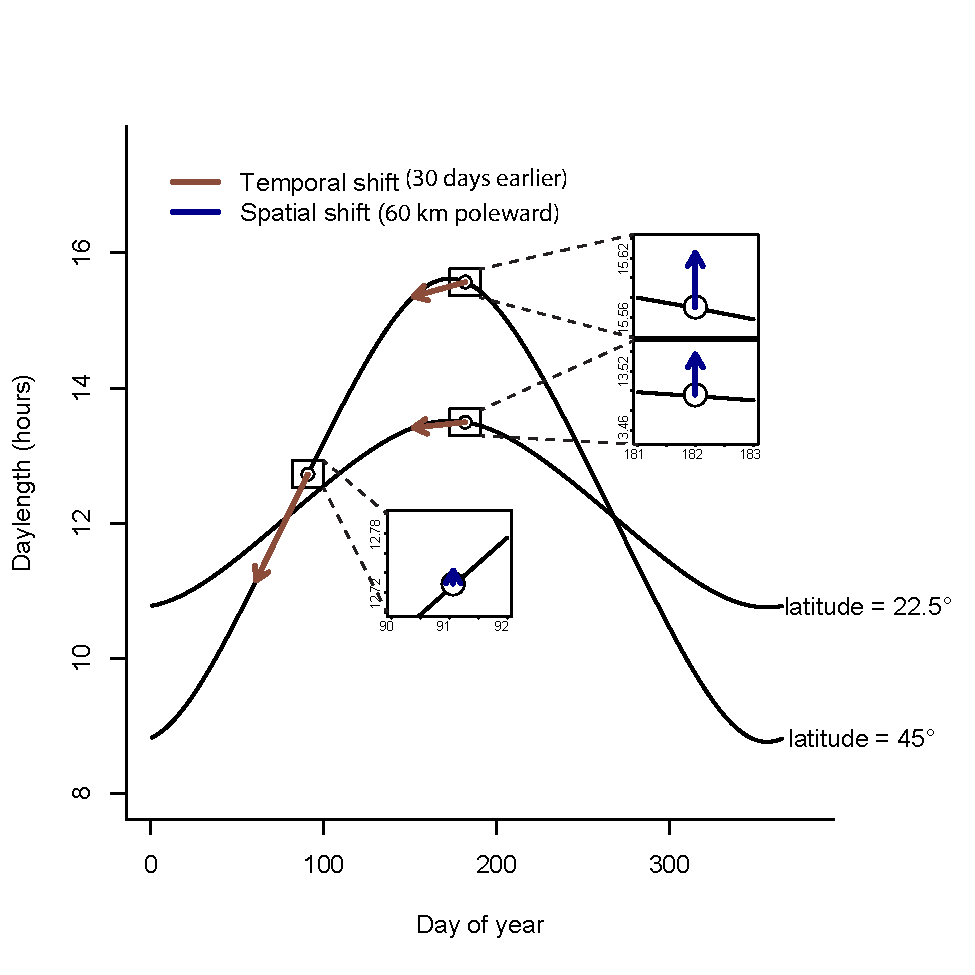
\includegraphics{/Users/aileneettinger/git/ospree/analyses/photoperiod/figures/photo_spacetime_v2.pdf} %
\caption{\textbf{Photoperiod varies with latitude and throughout the year}, such that temporal shifts in activity yield larger changes in experienced photoperiod compared with spatial shifts. Here, we show this variation at two latitudes, using hypothetical rates of spatial and temporal shifts: 30 days earlier for temporal shifts, and 0.5 degrees poleward for spatial shifts. These shifts, which are similar to observed average rates (e.g., Parmesan et. al 2006, Chen et al 2011), highlight the greater magnitude in daylength changes close to the equinox (e.g., DOY 91), versus close to the summer solcstice (e.g., DOY 182).}
 \label{fig:spacetime}%
 \end{figure}
 
\begin{figure}[p]
\centering
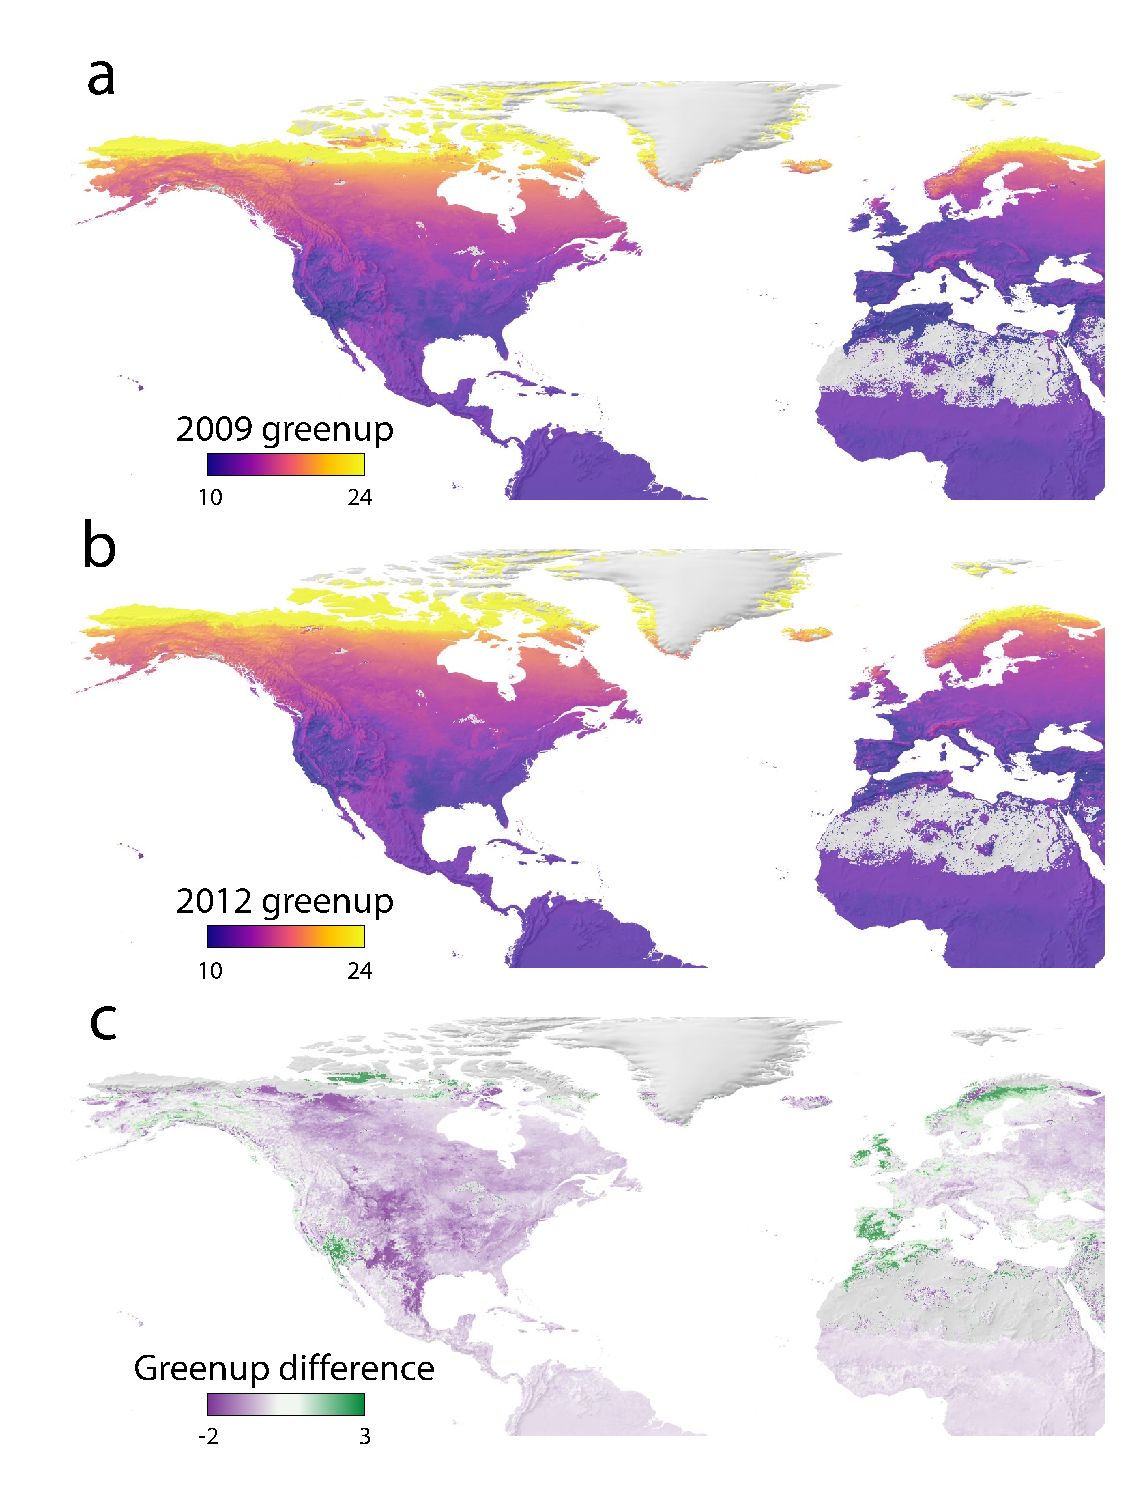
\includegraphics{/Users/aileneettinger/git/ospree/docs/photoperiod/figures/Greenup_.pdf} %2009 greenup
\caption{\textbf{The photoperiod on the green up date (start of spring) varies over space} and among years. Hours of daylight on the date of spring green up from MODIS satilite data across North America and Europe for an average (a) and  early (b) North American start of spring. The differences between the years are shown in (c). }
 \label{fig:greenup}%
 \end{figure}
\begin{figure}[p]
\centering
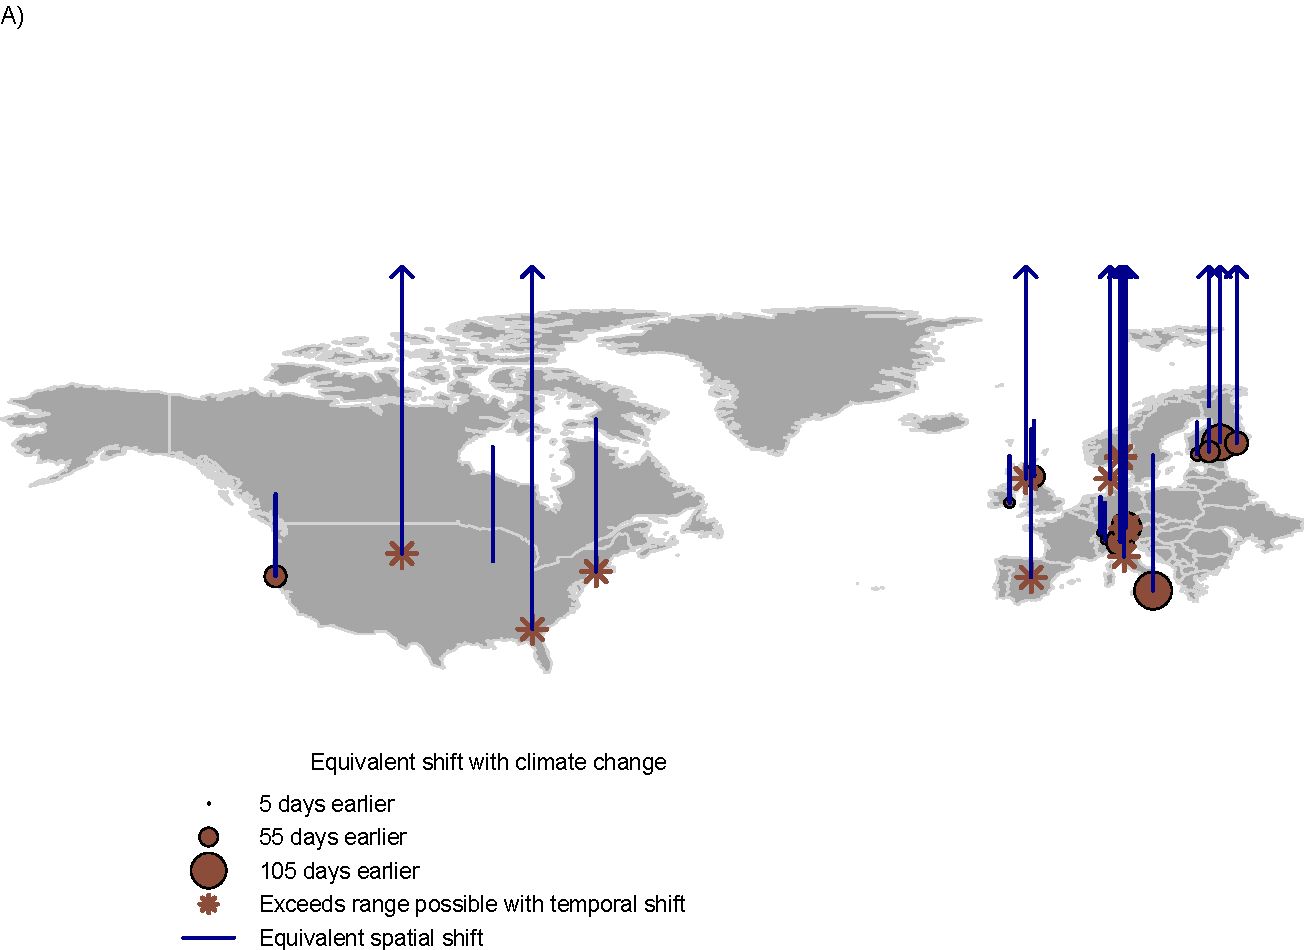
\includegraphics{/Users/aileneettinger/git/ospree/analyses/photoperiod/figures/ospree_photopmap.pdf} 
\caption{\textbf{OSPREE experiments that manipulate photoperiod}, and their equivalent spatial and temporal shifts, mapped (A), and graphed (B-C). Observed rates (dashed gray lines) 16.9 kilometers per decade (or approximately 1.5 degrees in 100 years) for spatial shifts (Chen et al. 2011) and 2.3 days per decade (or 23 days in 100 years) for temporal shifts (Parmesan and Yohe 2003).}
 \label{fig:photomap}
 \end{figure}


 
\begin{figure}[p]
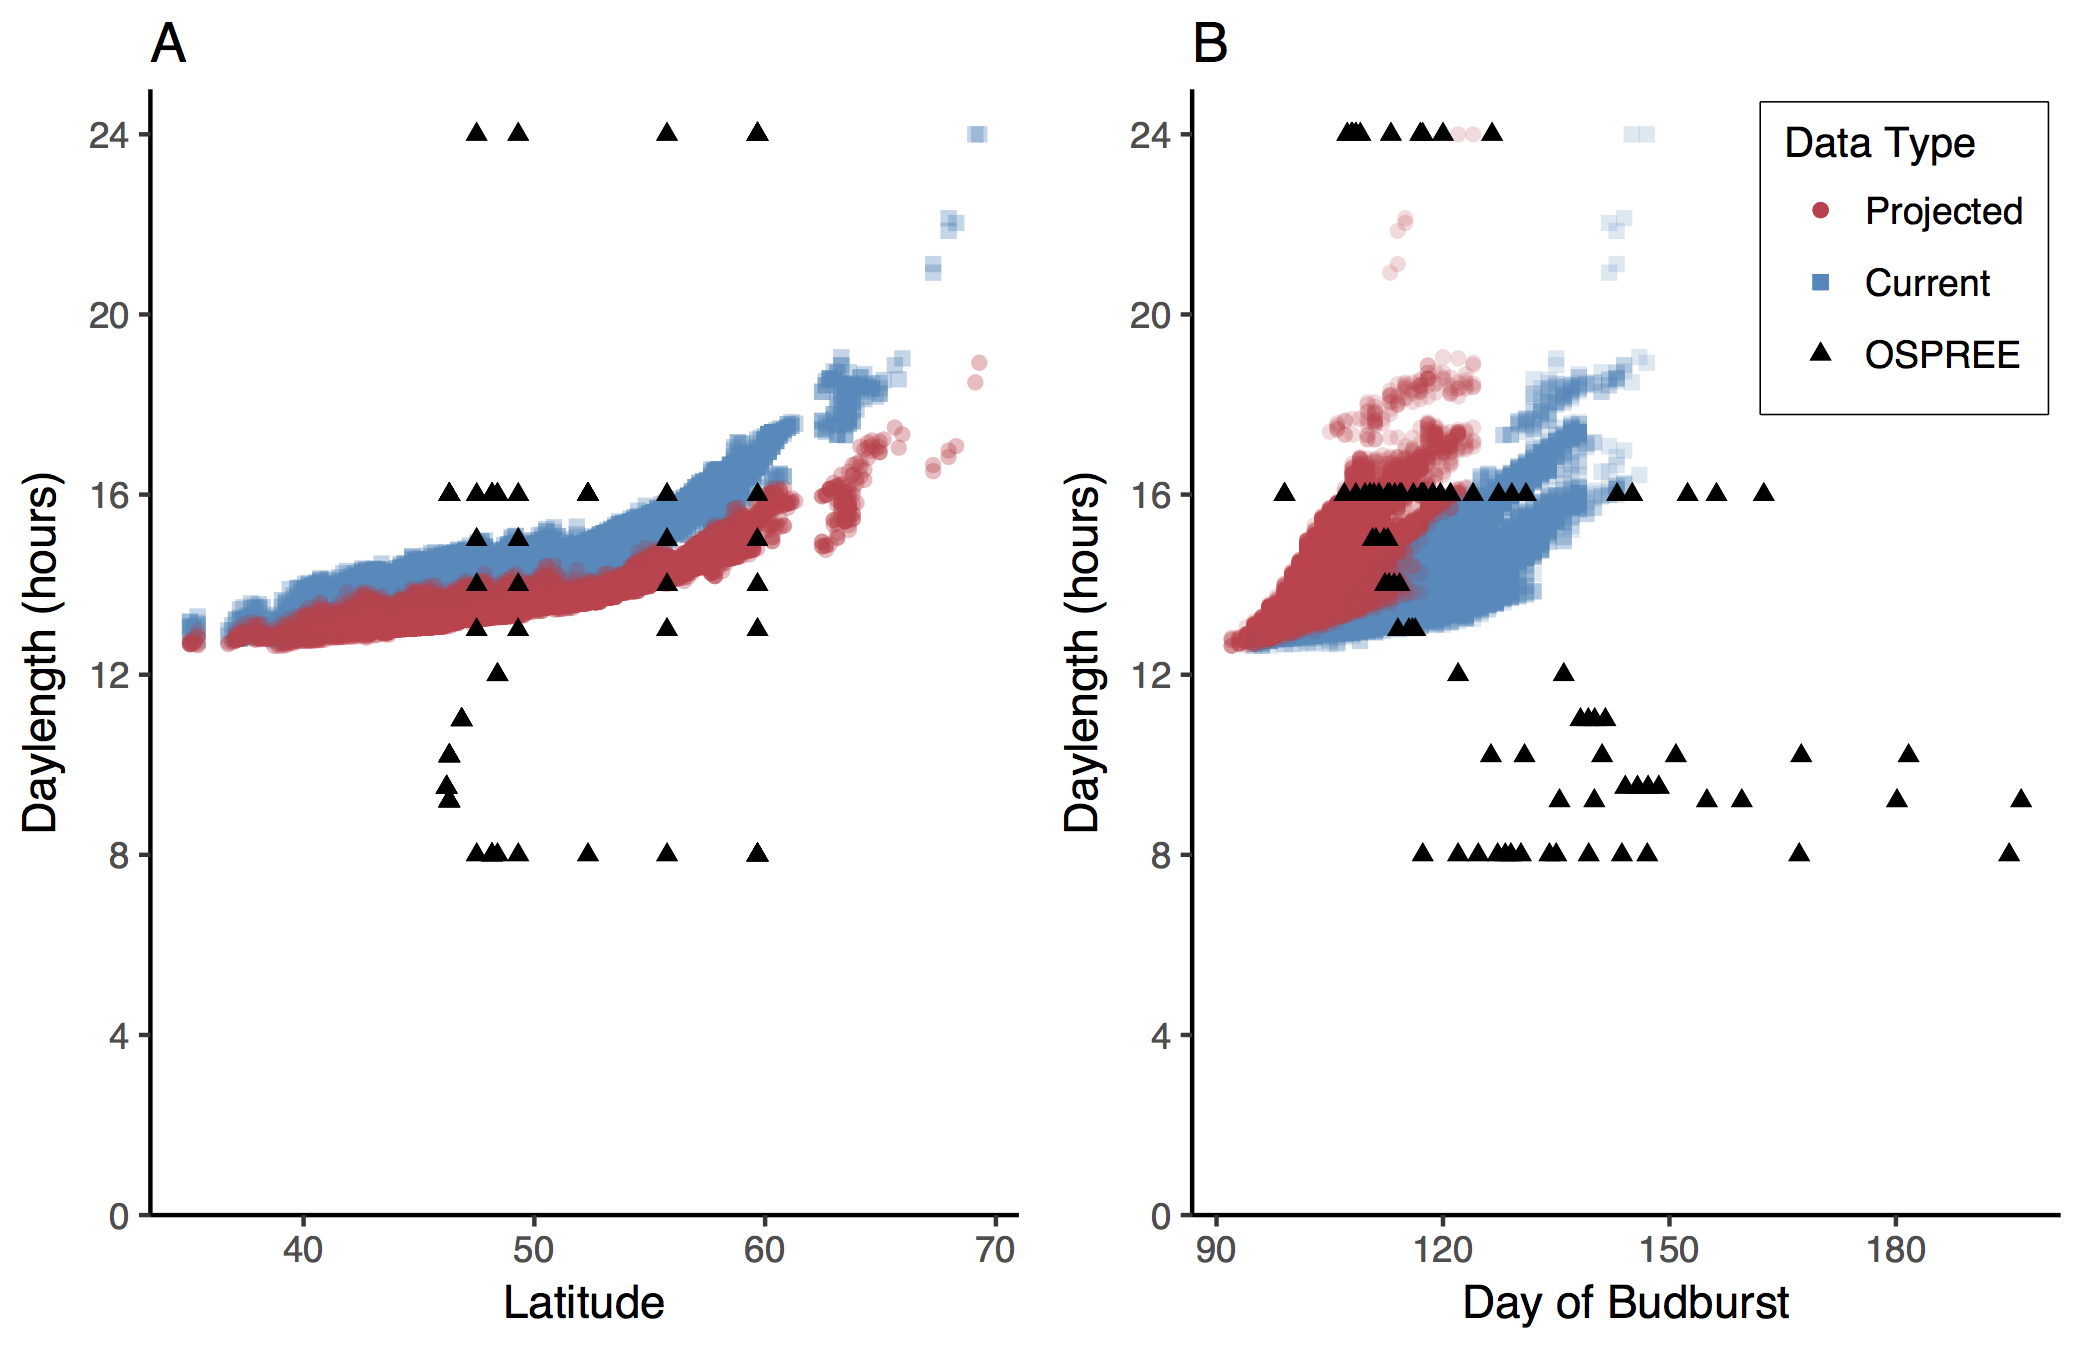
\includegraphics{/Users/aileneettinger/git/ospree/analyses/photoperiod/figures/2D_fagus_actual.png} 
\caption{\textbf{Experimental treatments of daylength in the OSPREE database, shown by latitude (A) and by day of budburst (B)} for \textit{Fagus sylvatica}. For comparison, we show the daylength when budburst occurs in its current and projected ranges (A) and in its current range only, with expected shifts in phenology (B). Estimates and projections are from Phenofit \citep{duputie2015}}
 \label{fig:fagus}
 \end{figure}
 
\begin{figure}[p]
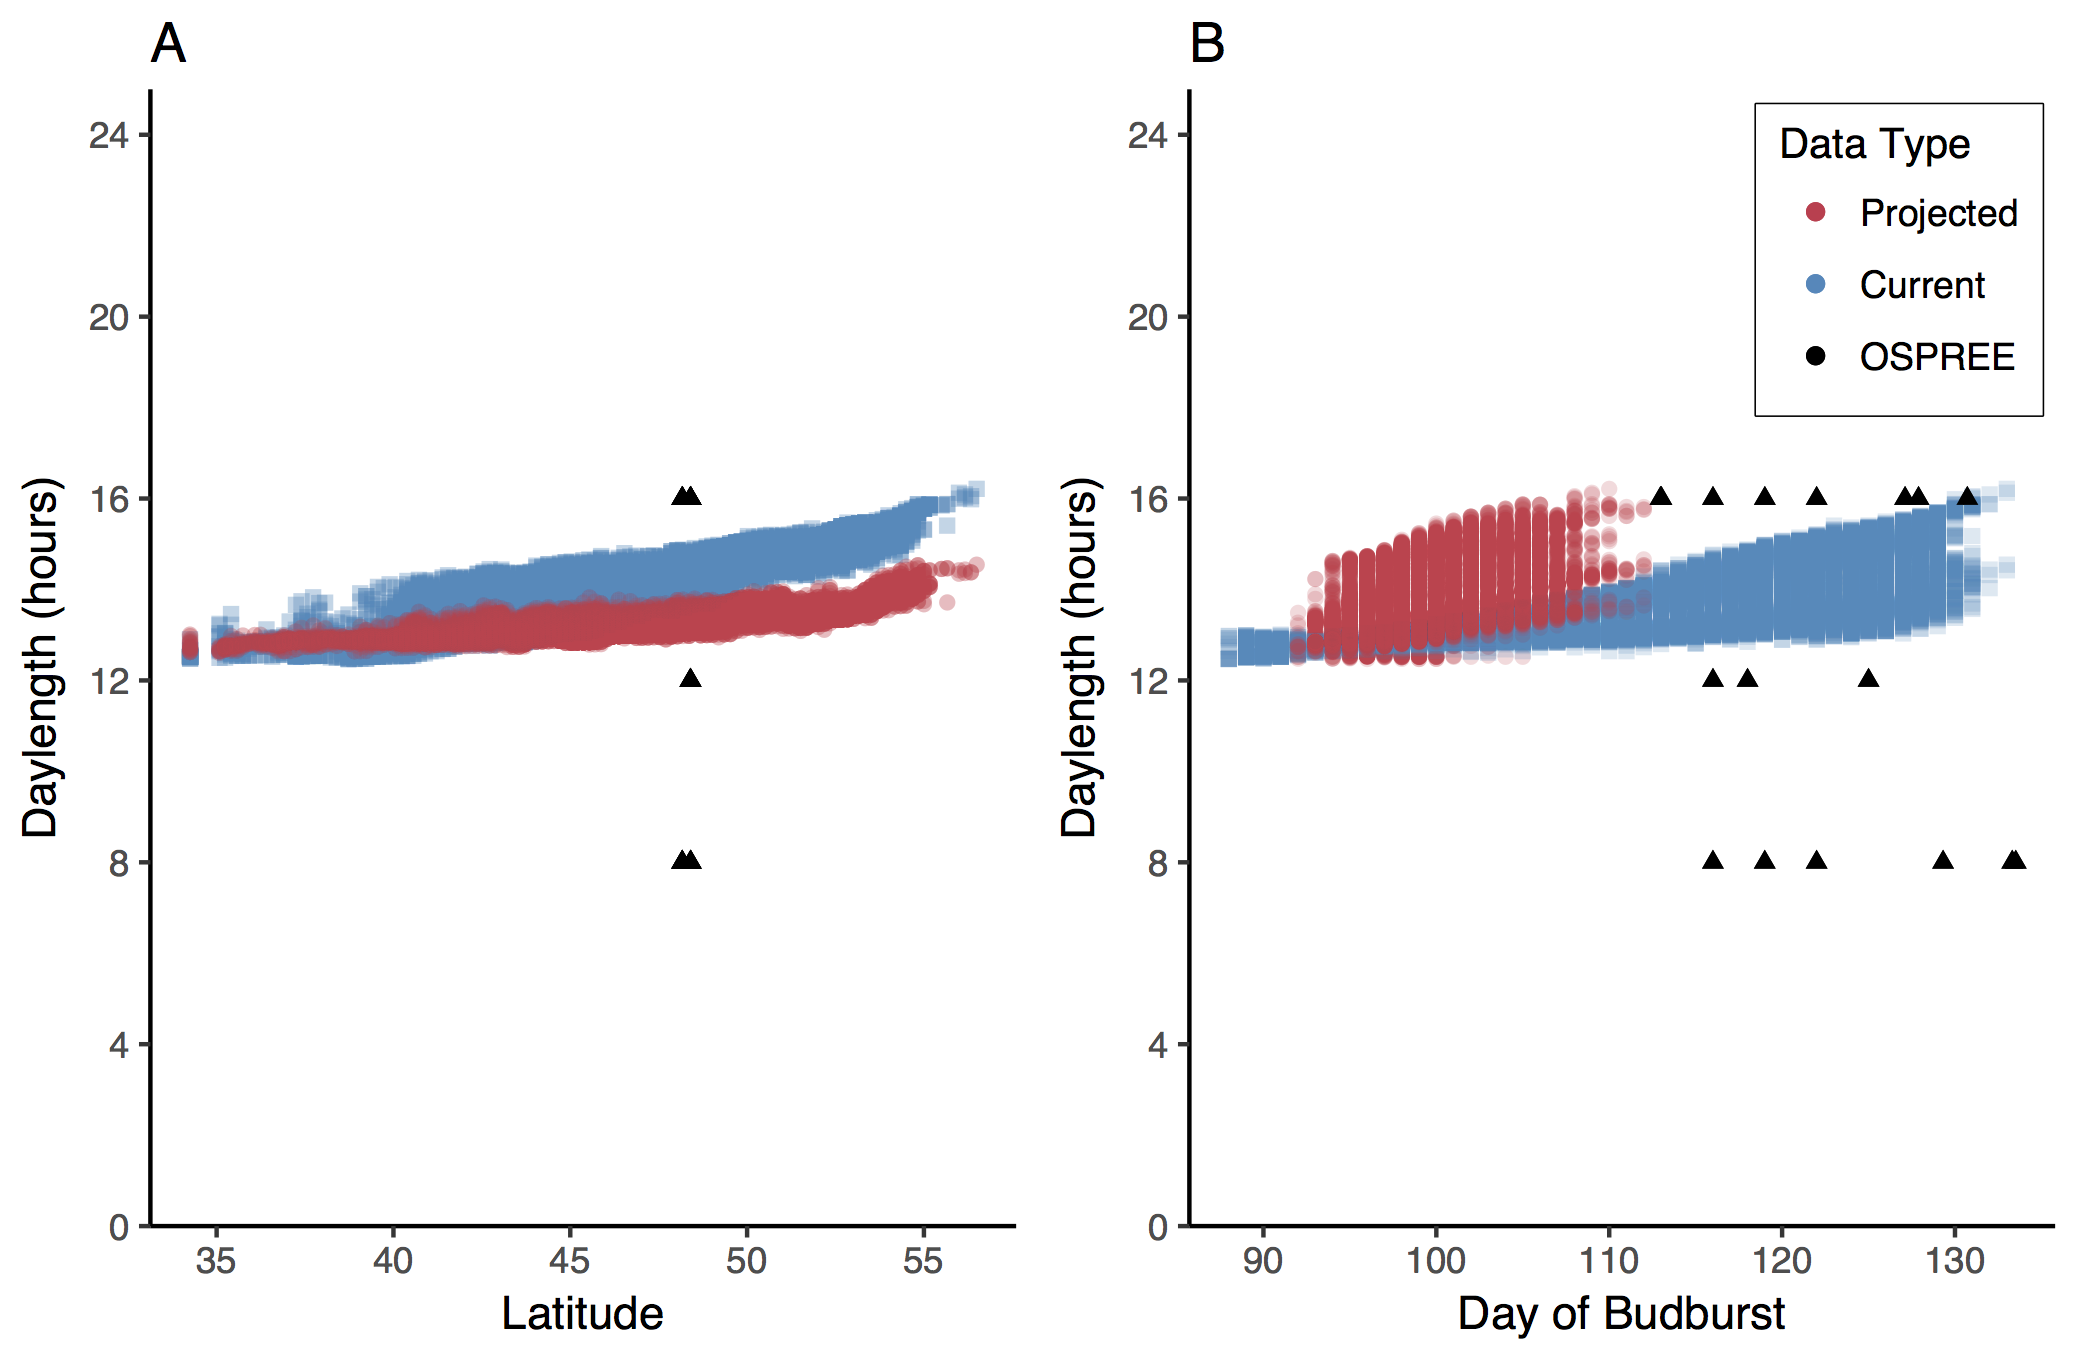
\includegraphics{/Users/aileneettinger/git/ospree/analyses/photoperiod/figures/2D_quercus_actual.pdf} 
\caption{\textbf{Experimental treatments of daylength in the OSPREE database, shown by latitude (A) and by day of budburst (B)} for \textit{Quercus robur}. For comparison, we show the daylength when budburst occurs in its current and projected ranges (A) and in its current range only, with expected shifts in phenology (B). Estimates and projections are from Phenofit \citep{duputie2015}.}
 \label{fig:quercus}
 \end{figure}
 
 \begin{figure}[p]
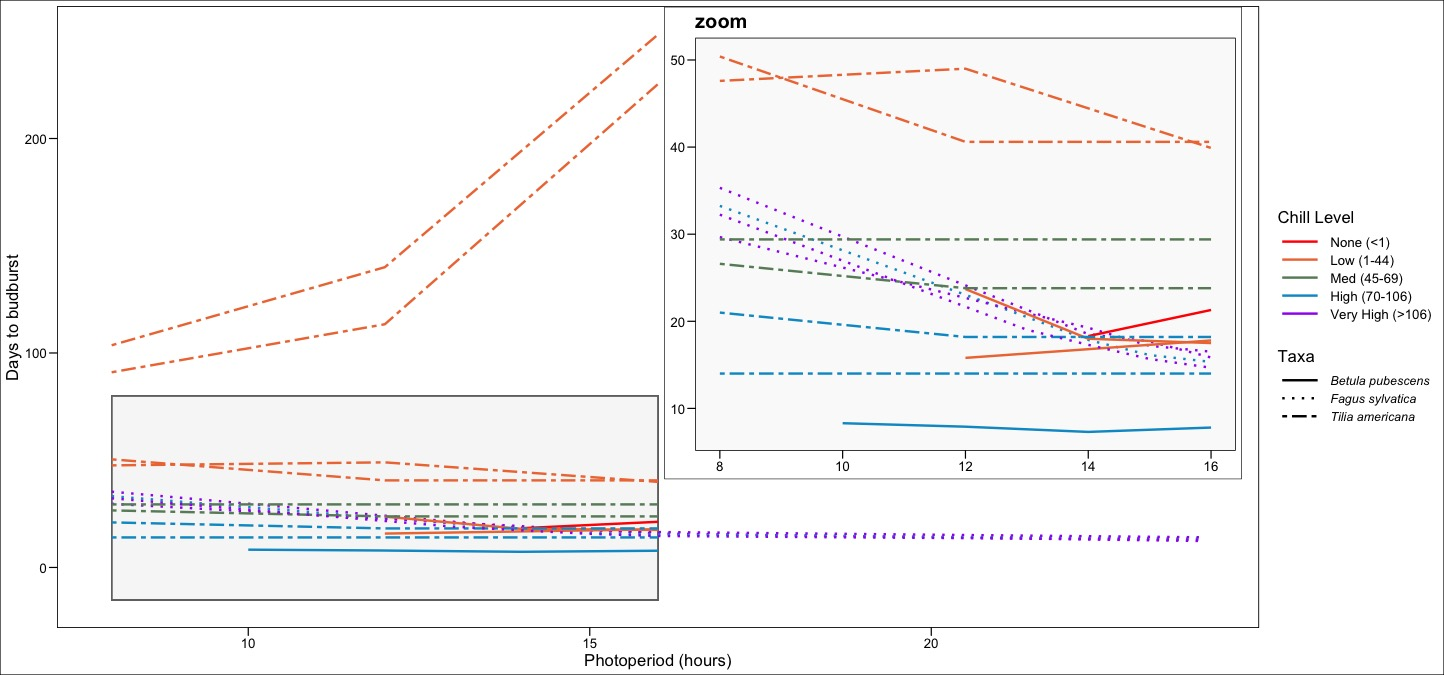
\includegraphics{/Users/aileneettinger/git/ospree/analyses/photoperiod/figures/Photo_curv_FINAL.jpeg} 
\caption{\textbf{Plant responses to changes in daylength vary across species and populations, and with the amount of chilling recieved}.}
 \label{fig:photocurve}
 \end{figure}
%%%%%%%%%%%%%%%%%%%%%%%%%%%%%%%%%%%%%%%%
\end{document}
%%%%%%%%%%%%%%%%%%%%%%%%%%%%%%%%%%%%%%%%
